\chapter{Методы многомерной минимизации}
\section{Основные определения}
Далее будем говорить про функции многих переменных, то есть однозначное соответствие $f(\vec x) = y$. Здесь $y$ - скаляр, а $\vec x$ - вектор столбец:
\begin{equation}
    \vec x = \left[
    \begin{array}{c}
         x_1  \\
         x_2  \\
         \vdots \\
         x_n
    \end{array}
    \right]
\end{equation}

Положительно определенной матрицей будем называть симметричную квадратную матрицу $a^T=a$, такую, что $f(\vec x) = {\vec x}^Ta{\vec x} > 0$ для любого $\vec x \neq \vec 0$. Для того, чтобы матрица была положительно определенной необходимо и достаточно, чтобы все собственные значения $\lambda$ данной матрицы были положительны, то есть при решении уравнения:
\begin{equation}
    \det \left( a_{ik} - \lambda\delta_{ik} \right)=0
\end{equation}
Здесь $\delta_{ik}$ - символ Кронекера, то есть:
\begin{equation*}
\delta_{ik} =
\left\{
\begin{array}{lr}
1 & \text{ для } i = k\\
0 & \text{ для } i \neq k
\end{array}
\right.
\end{equation*}
Пусть в многомерном пространстве $\vec x_0$ - первая точка, то есть точка с которой мы начинаем поиск минимума, а $\vec x^*$ - точка минимума функции. Алгоритм многомерной минимизации должен обеспечивать:
\begin{itemize}
    \item Направление движения к $\vec x^*$
    \item Задавать длину шага
\end{itemize}
Одной формулой требования к алгоритму можно задать так:
\begin{equation}
    \vec x_{k+1} =\vec x_k + \alpha_k \vec p
    \label{xk}
\end{equation}
Здесь $ \vec x_{k+1}$ следующая точка, получаемая с помощью алгоритма, $ \vec x_{k}$ - текущая точка, с которой производится переход в $ \vec x_{k+1}$, $\alpha_k$ - длина шага на $k$-ом этапе (скаляр) и $\vec p_k = \vec x_{k+1} - \vec x_{k} $ - вектор направления.

Гипотетически наша функция имеет аналитический вид, поэтому мы можем разложить ее в ряд Тейлора в некоторой окрестности точки $\vec x_k$:
\begin{equation}
    f(\vec x) = f(\vec x_k) + \alpha(f_{kc}',\vec p_k) + \frac{\alpha^2}{2}(f_{kc}'' \, \vec p_k,\vec p_k)
    \label{Teylor}
\end{equation}
Здесь стоит расписать обозначения, применимые в формуле (\ref{Teylor}):
\begin{equation*}
    f'_{kc} = \left[ 
    \begin{array}{c}
         \left.\frac{\partial f(\vec x)}{\partial x_1}\right|_{x_{kc_1}} \\
         \left.\frac{\partial f(\vec x)}{\partial x_2}\right|_{x_{kc_2}} \\
         \vdots \\
         \left.\frac{\partial f(\vec x)}{\partial x_n}\right|_{x_{kc_n}}
         \end{array}
    \right]^T
\end{equation*}
\begin{equation*}
    f_{kc}'' = \left[ 
    \begin{array}{cccc}
         \left.\frac{\partial^2 f(\vec x)}{\partial x_1^2}\right|_{x_{kc_1}} &
         \left.\frac{\partial^2 f(\vec x)}{\partial x_1 \partial x_2}\right|_{x_{kc_1}} &
         \ldots &  \left.\frac{\partial^2 f(\vec x)}{\partial x_1 \partial x_n}\right|_{x_{kc_1}} \\
         \left.\frac{\partial^2 f(\vec x)}{\partial x_2 \partial x_1}\right|_{x_{kc_2}} &
         \left.\frac{\partial^2 f(\vec x)}{\partial x_2^2}\right|_{x_{kc_2}} &
         \ldots &  \left.\frac{\partial^2 f(\vec x)}{\partial x_2 \partial x_n}\right|_{x_{kc_2}} \\
         \vdots & \vdots & \ddots & \vdots \\
         \left.\frac{\partial^2 f(\vec x)}{\partial x_n \partial x_1}\right|_{x_{kc_n}} &
         \left.\frac{\partial^2 f(\vec x)}{\partial x_n \partial x_2}\right|_{x_{kc_n}} &
         \ldots &  \left.\frac{\partial^2 f(\vec x)}{\partial x_n^2}\right|_{x_{kc_n}}
    \end{array}
    \right]
\end{equation*}
Дифференцирование в точке $\vec x_k$ фактически означает дифференцирование в окрестности, близ точки  $\vec x_k$, то есть типа в интервале $[x_k, x_{kc}]$, где $x_{kc}$ точка, значение которой дается формулой:
\begin{equation*}
   \vec x_{kc} =\vec x_k + \theta\left(\vec x - \vec x_k\right) \qquad \theta \epsilon [0; 1]
\end{equation*}

Так как мы ищем минимум при условии, что движение направлено к точке минимума, то $f(\vec x_{min}) < f(\vec x_k) < f(\vec x_0)$, где $\vec x_{min}$ - точка фактического минимума функции. 

Считаем, что разложение происходит настолько близко к точке $\vec x_{min}$, что функция является невыпуклой, а значит матрица второй производной положительно определена, что дает нам сделать утверждение о знаке второго члена разложения ряда (\ref{Teylor}). Поскольку, как мы говорили выше, для положительно определенной матрицы $\left(f_{kc}'' \, \vec p_k,\vec p_k\right) > 0$, а $\frac{\alpha^2}{2} \geqslant 0$, то получается, что слагаемое второго порядка положительно. Но так как есть необходимость в том, чтобы в точке, ближней к точке фактического минимума функции ($f(\vec x) < f(\vec x_k)$), то слагаемое первого порядка $\alpha(f_{kc}',\vec p_k) < 0$, что подводит нас к первому методу многомерной минимизации.

\section{Градиентный метод} \label{GradientMethod}
В данном методе в качестве $\vec p_k$ просто берется выражение $-f'(\vec x_k) = -f'_k$. Тогда выражение (\ref{xk}) примет вид:
\begin{equation}
    \vec x_{k+1} = \vec x_k - \alpha_k f'(\vec x_k) \textbf{, } \quad \alpha_k > 0 \text{, } k = 0, 1 \ldots
\end{equation}
Выбором такого значения $\vec p_k$ мы определили направление движения, а также уменьшения функции при приближении к точке $(f'(\vec x_k), p) < 0$. Осталось найти шаг $\alpha_k$, где $k$ -индекс итерации.

Рассмотрим процесс выбора шага на примере.
Пусть рассматриваемая функция имеет аналитическое выражение:\
\begin{equation}
    f(x,y) = \frac12\left(\frac{x^2}{a^2} + \frac{y^2}{b^2}\right)
    \label{ellipse}
\end{equation}
\begin{figure}
    \centering
    \begin{tikzpicture}[scale = 4,
axis/.style = {very thick, <->, >=stealth'},
dashed line/.style = {dashed, very thick},
plane line/.style = {very thick, color = brown}]
\tikzset{mypoints/.style={fill=white,draw=black,thick}}
\def\aa{30} \def\ba{15} \def\ab{20} \def\bb{10} \def\ac{10} \def\bc{5}
\draw[axis] (2, 0) node[right]{$x$} -- (0, 0) -- (0, 1) node[above]{$y$};
\draw[dashed](-2, 0) -- (0, 0) -- (0,-1);
\fill[mypoints] circle (2pt);
\fill[black] (0, 0) circle (1pt) node[below, shift={(0:20pt)}]{$f\left(x,y\right)$};
\draw[name path=ellipse,red,very thick]
		(0,0) circle[x radius = \aa pt, y radius = \ba pt];
\draw[name path=ellipseb,blue,very thick]
		(0,0) circle[x radius = \ab pt, y radius = \bb pt];
\draw[name path=ellipsec,green,very thick]
		(0,0) circle[x radius = \ac pt, y radius = \bc pt];
\draw[name path = plane_a ,plane line] (0, -0.85) -- (1.5, .1);
% \coordinate[label=right:$(x_0, y_0)$] (xo) at (intersection of (0, -0.85) -- (1.5, .1) and ellipse); 
\path [name intersections={of = ellipse and plane_a}];
\coordinate (X0) at (intersection-1);
\fill[mypoints] (X0) +(-0.95cm, +1.5cm) coordinate (Xend) circle (0pt) ;
\fill[mypoints] (X0) +(-0.3166cm, +.5cm) coordinate (X1) circle (0pt) ;
\fill[mypoints] (X1) +(-0.2cm, -.2cm) coordinate (X2) circle (0pt) ;
\draw[->, very thick, color = brown] (X0) -- (Xend);
\fill[mypoints] (X0) circle (1pt) node[right, shift={(0:15pt)}]{$(x_0, y_0)$};
\fill[mypoints] (X1) circle (1pt) node[right]{$(x_1, y_1)$};
\node[anchor=west,text width=6cm] at (-2, 1){\textcolor{red}{$f(x,y)$}$>$\textcolor{blue}{$f(x,y)$}$>$\textcolor{green}{$f(x,y)$}} ;
    \end{tikzpicture}
    \caption{Иллюстрация первого шага метода антиградиента}
    \label{fig:antigradient}
\end{figure}
На рисунке \ref{fig:antigradient} разными цветами показаны линии уровня эллипсоида. Линия уровня соответствует какому-то значению функции во всех ее точках. Так, значение в красном сечении эллипсоида больше чем в синем, а то, в свою очередь, больше чем в зеленом. Предположим, что мы выбрали точку $(x_0, y_0)$ на поверхности эллипсоида. Проведем линию уровня в этой точке, то есть линию, которая получалась бы, если бы мы <<отрезали>> кусок эллипсоида в этой точке перпендикулярно оси значений функции ($f(x,y)$). Далее в этой линии уровня проводим касательную в этой точке. Градиент функции в этой точки всегда будет перпендикулярен касательной. Так как метод призван искать минимум функции, то направление движения стоит выбирать к минимуму, а значит со знаком минус. На рисунке коричневой стрелкой показано направление движения в поисках минимума. 

Как же выбрать шаг? В сечении направления движения мы получаем кривую второго порядка. Останавливаться стоит тогда, когда достигнут минимум этой кривой.. То есть, допустим мы рассекли эллипсоид и получили нечто вроде параболы в этом сечении. Значит минимум этой параболы и будет следующей точкой, где будет повторяться описанная выше процедура. На рисунке \ref{fig:antigradient} эта точка обозначена $(x_1, y_1)$. После ее нахождения получаем новую линию уровня, проводим новую касательную и т. д. Процесс повторяется до тех пор, пока будет условие, где $\varepsilon$ мы задаем сами.:
\begin{equation}
    \frac{f(\vec x_{k+1}) - f(\vec x_k)}{f(\vec x_k)} > \varepsilon
    \label{ag_stop}
\end{equation}
 
\section*{Вопрос}
В каком случае метод антиградиента справится с функцией \ref{ellipse} за один шаг, а в каком, возможно, вовсе не справится?
\section*{Ответ}
В случае если $a=b$. Тогда, полученная поверхность это сфера. При получении любой линии уровня - в сечении будет окружность, а значит направление антиградиента всегда будет к центру этой окружности. Сечение, проходящее через центр окружности, будет пересекать и минимум сферы, а значит первый же шаг приведет нас в минимум функции.

В случае $a\ll b$ или $a \gg b$ одна ось эллипсоида будет вытянута относительно другой достаточно сильно. Если мы начнем наши измерения с точки, далекой от центра и антиградент в которой не будет сразу проходить через центр, то мы будем идти к минимуму достаточно долго, или условие (\ref{ag_stop}) выполнится гораздо раньше, чем мы достигнем минимума.

На этом примере мы видим, что метод антиградиента не так хорош, однако, путем замены координат, этот случай можно свести к обыкновенной сфере, с чем, как мы убедились, градиентный метод с легкостью справится. Тут возникает одно из условий для использования метода: Необходимо, чтобы масштаб осей был соразмерным, то есть изменение по одной оси на 1 не приводило к изменению по другой оси на, скажем, 1000. 

Вообще говоря, главный недостаток метода антиградента состоит в том, что он не чувствителен к перпендикулярным направлениям. То есть сечение функции по направлению наибольшего спада не учитывает значения функции в некоторой окрестности кривой сечения. Однако следующий метод лишен данного недостатка.


\section{Метод Ньютона с регулировкой шага} \label{NewtMeth}
Возьмем гипотетическое разложение исследуемой функции $f(\vec x)$ в ряд Тейлора в точке $\vec y$ с точностью до второго порядка и обозначим его через $\psi(\vec x)$:
\begin{equation}
    \psi(\vec x) = f(\vec y) + \left(f'(\vec y), \vec x - \vec y\right) + \frac12\left(f''(\vec y)(\vec x - \vec y), (\vec x - \vec y)\right)
\end{equation}
Минимизация данного выражения (путем нахождения минимума) дает оптимальное значение вектору $\vec p$:
\begin{equation}
    \vec p= \vec x - \vec y = - \left(f''(\vec y)\right)^{-1}f'(\vec y)
    \label{p_newton}
\end{equation}
Проверим условие для движения к минимуму, которое было представлено в подразделе введения $\left(f'(\vec y), \vec p\right) < 0$. Умножаем слева выражение (\ref{p_newton}) на матрицу Гессе ($f''(\vec y)$):
\begin{equation}
    f''(\vec y)\vec p = - f'(\vec y)
\end{equation}
Умножаем это выражение справа на $\vec p$ и убеждаемся в действительности условия:
\begin{equation}
    0<\left(f''(\vec y)\vec p, \vec p\right) = - \left(f'(\vec y), \vec p\right)
\end{equation}
Тогда выражение (\ref{xk}) становится:
\begin{equation}
    \vec x_{k+1} = \vec x_k - \alpha_k (f''(\vec x_k))^{-1} f'(\vec x_k) \textbf{, } \quad \alpha_k > 0 \text{, } k = 0, 1 \ldots
\end{equation}
Если $\alpha_k = const$ для любой $k$, то данный метод называется метод Ньютона. В случае, если $\alpha_k \neq const$ при любом $k$, то метод называется методом Ньютона с регулировкой шага.
\section{Метод Дэвидона-Флетчера-Пауэлла}
Мы увидели, что в отличие от метода антиградиента, метод Ньютона <<Умеет смотреть по сторонам>>, путям взятия матрицы второй производной, а значит определения выпуклости функции в точке. Однако, учитывая специфику данного метода, существует необходимость взятия обратной матрицы от матрицы вторых производных (матрицы Гессе), что, вообще говоря, не всегда является корректной задачей, поскольку процедура обращения матрицы неустойчива. Поэтому возникла идея создать такой метод, в которым нет необходимости вычислятьобратную матрицу Гессе.

Алгоритм автоматически синтезирует метод антиградиента и метод Ньютона. Происходит это за счет того, что процедура поиска минимума начинается градиентным методом, описанным в подразделе \ref{GradientMethod}, и заканчивается методом Ньютона (\ref{NewtMeth}).
В этом случае выражение \ref{xk} имеет следующий вид:
\begin{equation}
    \vec x_{k+1} = \vec x_k - \lambda_k \eta(\vec x_k)f'(\vec x_k)
\end{equation}
где $\eta(\vec x_k)$ - матрица направлений, $\lambda_k$ - длина шага.
Сущность метода антиградиента проявляется только на первом шаге. В этот момент матрица направлений эквивалентна единичной матрице, размерности $n$, где количество параметров функции:
\begin{equation*}
    \eta (x_0) = \hat I = \left[\begin{array}{cccc}
        1 & 0 & \ldots & 0 \\
        0 & 1 & \ldots & 0 \\
        \vdots & \vdots & \ddots & \vdots\\
        0 & 0 & \ldots & 1
    \end{array}\right]
\end{equation*}
А в точке минимума матрица направлений должна совпадать с матрицей обратной матрице Гессе, то есть:
\begin{equation*}
    \eta(x_{min}) = \left(f''(x_{min})\right)^{-1}
\end{equation*}
Вторая производная в дискретных функциях может вычисляться следующим образом, поскольку мы не располагаем аналитическим видом функции, а значит не можем пользоваться классическим определением производной через пределы:
\begin{equation}
    f'(\vec x_{k+1})-f'(\vec x_k) \approx f''(\vec x_k)(\vec x_{k+1}-\vec x_k)
    \label{deriv}
\end{equation}
Домножаем (\ref{deriv}) слева на обратную матрицу Гессе и получаем:
\begin{equation}
    \Delta \vec x_k=\vec x_{k+1}-\vec x_k \approx \left(f''(\vec x_k)\right)^{-1}\left(f'(\vec x_{k+1})-f'(\vec x_k)\right) =  \left(f''(\vec x_k)\right)^{-1}\Delta g_k
\label{delta_x}
\end{equation}
Хотим, чтобы $ \left(f''(\vec x_{k+1})\right)^{-1}$ была пропорциональна матрице направлений на $k+1$ шаге. Более того, хотим, чтобы матрица направлений менялась от шага к шагу аддитивно, то есть:
\begin{equation}
    (f''(\vec x_{k+1}))^{-1} \approx w\eta(\vec x_{k+1}) \approx w(\eta(\vec x_k)+\Delta \eta (\vec x_k))
    \label{ita}
\end{equation}
Здесь $\omega$ - коэффициент пропорциональности. Тогда, учитывая (\ref{delta_x}) и (\ref{ita}):
\begin{align}
    \eta_{k+1}\Delta g_k & {}= \frac1{\omega}\Delta \vec x_k \\
    \Delta \eta_{k} \Delta g_k & {} =
    \frac1{\omega} \Delta \vec x_k - \eta_k \Delta g_k
    \label{delta_eta}\end{align}
Если рассматривать это выражение как уравнение относительно $\Delta \eta_k$, то его решение:
\begin{equation}
    \Delta \eta_k = \frac1{\omega}\frac{\Delta\vec x_k {\vec y}^T}{{\vec y}^T \Delta g_k} - \frac{\eta_k \Delta g_k {\vec z}^T}{{\vec z}^T \Delta g_k}
    \label{solve_eta}
\end{equation}
Здесь $\vec z$ и $\vec y$ - произвольные вектора.

Если решение (\ref{solve_eta}) подставить в (\ref{delta_eta}), то получим тождество. Поскольку вектора $\vec z$ и $\vec y$ произвольные, то можем положить:
\begin{equation}
    \vec y_k = \Delta \vec x_k \text{;} \qquad \vec z_k = \eta_k \Delta g_k
\end{equation}
Чтобы $\eta_{k+1}$ получилась равной обратной матрице Гессе на $k$-м шаге.

Напишем алгоритм для вычисления минимума методом Дэвидона.

Чтобы программа по нахождению минимума остановилась, нужно, чтобы одновременно выполнились следующие условия:
\begin{equation}
    \frac{f(\vec x_{k+1}) - f(\vec x_k)}{f(\vec x_k)} < \varepsilon_1
\end{equation}
\begin{equation}
    \frac{\Delta \vec x_i^{(k)}}{\vec x_i^{(k)}} < \varepsilon_{2}^{(i)}
\end{equation}
\section{Сравнение алгоритмов многомерной минимизации}
Алгоритм многомерной минимизации должен отвечать следующим критериям:
\begin{enumerate}
    \item Метод работает для широкого спектра функций. Универсальность метода.
    \item Число необходимых вычислений целевой функции чем меньше тем лучше. Например вычисление одной производной требует 2 вычисления значения функции в разных точках, а второй производной целых 3 значения.
    \item Чем меньше количество итераций для достижения минимума с определенной точностью, тем лучше.
\end{enumerate}

Классическая тестовая задача для проверки алгоритмов многомерной минимизации - функция Розенброка (рис. \ref{fig:Rosenbrock}):
\begin{equation*}
    f(\vec x) = 100 (x_2 - x_1^2)^2 +(1-x_1)^2
\end{equation*}
Известно, что:
\begin{equation}
    \vec x_{min} = \left[\begin{array}{cc}
        1 \\
        1 
    \end{array}\right]\text{;} \qquad f(x_{min}) = 0
\end{equation}
\begin{figure}
    \centering
    \includegraphics[scale = 0.7]{Pictures/Rosenbrock.png}
    \caption{Функция Розенброка в трехмерном виде}
    \label{fig:Rosenbrock}
\end{figure}
\textit{По аналитическому виду функции можно заметить, что масштаб осей не соразмерен, о чем мы говорили разделе \ref{GradientMethod}}
%Надо изобразить функцию Розенброка

Посмотрим как справятся изученные нами методы с этой функцией (рис. \ref{fig:Rosenbrock_levels}):
\begin{figure}
    \centering
    \includegraphics[scale = 0.5]{Pictures/Rosenbrock_levels.png}
    \caption{Линия уровней функции Розенброка. Иллюстрация к сравнению методов.}
    \label{fig:Rosenbrock_levels}
\end{figure}
\begin{enumerate}
    \item Для метода антиградиента может не выйти найти минимум такой функции. Это зависит от первой точки, которая будет выбрана. Минимума мы можем не достичь поскольку первым шагом мы попадем на <<дно>>, где функция уже мало меняется, и не выполняются критерии продолжения алгоритма. Попасть в минимум сможем только если первое направление пройдет через точку минимума непосредственно. Эта ситуация показывает нам еще один критерий сравнения, а именно независимость от точки старта.
    \item Для метода Ньютона на первом же шаге направление будет отличаться от направления первого шага метода антиградиента, поскольку вторая производная дает методу <<зрение>>. Метод хорошо справляется с тестовой функцией.
    \item Очевидно, что метод Дэвидона тоже справится с такой функцией, поскольку это синтез первых двух методов.
\end{enumerate}
Все программы имеют критерии останова, которые подразумевают, что мы приблизились к минимуму, с достаточной точностью. Однако на деле это не всегда так. Ниже перечислены случаи, когда это утверждение ложно:
\begin{enumerate}
    \item Достижения требуемой окрестности минимума. То есть условия выхода слишком лояльные.
    \item Достигнут локальный минимум. Чтобы избавиться от этого достаточно примерно знать окрестность глобального минимума или повторить процедуру с другой начальной точкой.
    \item Алгоритм толчется на одном месте.
\end{enumerate}

 Однако существуют функции (поверхности) об которые сломается любой из этих алгоритмов. Достаточно посмотреть на рисунки \ref{fig:Bad_surfaces}. Их общая проблема заключается в том, что большая часть функции является просто плоскостью, поэтому здесь алгоритмы минимизации будут бесполезны - программа не сдвинется с места. Однако используя методы Монте-Карло можно <<бросать точку>> по всей поверхности много раз и определить окрестность, в которой функция отлична от константы. В левом рисунке проблема также заключается в том, что в фактическом минимуме функции не существует производной, поэтому рано или поздно двигаясь к минимуму алгоритм сломается.
 \begin{figure}
    \centering
    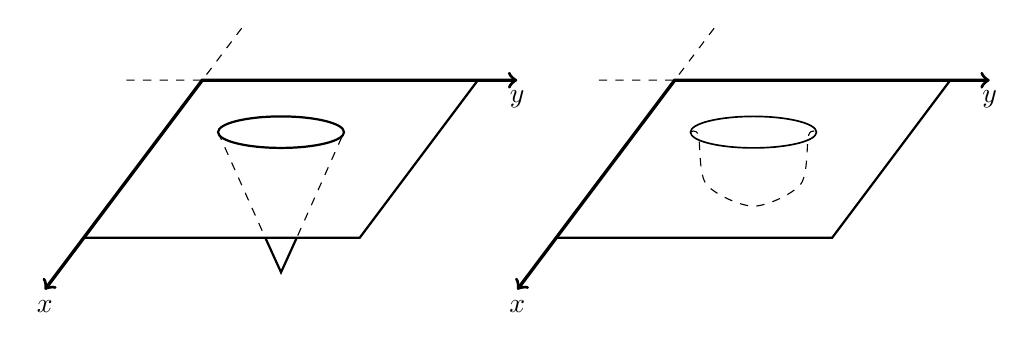
\begin{tikzpicture}
    [scale = 2,
    axis/.style = {<->, very thick},
    dashed line/.style={dashed, thick}]
    \draw[axis](3, 0)node[below]{$y$} -- (1, 0) -- (0, -1.33)node[below]{$x$};
    \draw[dashed](1.25, 0.33) -- (1, 0) -- (0.5, 0);
    \draw[thick](.25, -1) -- (2, -1) -- (2.75, 0);
    \draw[thick] (1.5, -0.33) ellipse (.4 and 0.1);
    \draw[dashed] (1.1, -0.33) -- (1.4, -1) -- (1.6, -1) -- (1.9, -0.33);
    \draw[thick] (1.4, -1) -- (1.5, -1.22) -- (1.6, -1);
    
    \draw[axis](6, 0)node[below]{$y$} -- (4, 0) -- (3, -1.33)node[below]{$x$};
    \draw[dashed](4.25, 0.33) -- (4, 0) -- (3.5, 0);
    \draw[thick](3.25, -1) -- (5, -1) -- (5.75, 0);
    \draw[semithick] (4.5, -0.33) ellipse (.4 and 0.1);
    \draw [dashed] plot [smooth] coordinates {(4.1,-0.33) (4.15, -0.35) (4.2,-0.66) (4.5,-.8) (4.8,-0.66) (4.85, -0.35) (4.9,-0.33)};
    \end{tikzpicture}
    \caption{Поверхности, с которыми методы многомерной минимизации не справятся}
    \label{fig:Bad_surfaces}
\end{figure}
 %Ниже приведу рисунки
 
 \textit{Для экономии вычислительных мощностей и времени работы алгоритмов в физике принято ограничивать значения переменных и функции, в пределах которых ищется минимум.}
